\documentclass[12pt,a4paper]{article}
\usepackage[margin=2.2cm]{geometry}
\usepackage{ctex}
\usepackage{amsmath,amssymb,amsfonts}
\usepackage{graphicx}
\usepackage{tikz}
\usetikzlibrary{calc,positioning,arrows.meta,decorations.pathreplacing,matrix}
\usepackage{booktabs}
\usepackage{enumitem}
\usepackage{xcolor}
\usepackage{tcolorbox}
\usepackage{hyperref}
\usepackage{float}
\usepackage{array}

\tcbuselibrary{theorems,skins,breakable}

\definecolor{myblue}{RGB}{0,102,204}
\definecolor{myred}{RGB}{204,0,0}
\definecolor{mygreen}{RGB}{0,153,0}
\definecolor{mypurple}{RGB}{128,0,128}
\definecolor{myorange}{RGB}{230,120,0}
\definecolor{lightblue}{RGB}{220,235,255}
\definecolor{lightyellow}{RGB}{255,255,220}
\definecolor{lightgreen}{RGB}{220,255,220}
\definecolor{lightred}{RGB}{255,225,225}
\definecolor{lightpurple}{RGB}{240,225,255}

\newtcolorbox{keybox}[1][]{
  colback=lightblue, colframe=myblue,
  fonttitle=\bfseries, title={#1},
  breakable
}

\newtcolorbox{exbox}[1][]{
  colback=lightyellow, colframe=myorange,
  fonttitle=\bfseries, title={#1},
  breakable
}

\newtcolorbox{warnbox}[1][]{
  colback=lightred, colframe=myred,
  fonttitle=\bfseries, title={#1},
  breakable
}

\newtcolorbox{sumbox}[1][]{
  colback=lightgreen, colframe=mygreen,
  fonttitle=\bfseries, title={#1},
  breakable
}

\newtcolorbox{notebox}[1][]{
  colback=lightpurple, colframe=mypurple,
  fonttitle=\bfseries, title={#1},
  breakable
}

\title{\Huge\textbf{N 皇后问题的转移矩阵构造法} \\ \Large 从 $A$ 矩阵到 T 张量的优雅推导}
\author{张量网络学习笔记}
\date{2026年3月}

\begin{document}

\maketitle
\tableofcontents
\newpage

%=============================================================================
\section{引言：为什么需要新方法？}
%=============================================================================

在之前的学习笔记中，我们用一个 9 阶张量 $B(u, ul, l, ld, d, dr, r, ru, p)$ 来编码 N 皇后问题的局部约束。该张量有 $2^9 = 512$ 个元素，其中 17 个非零（16 个空格子状态 + 1 个皇后状态），需要\textbf{逐个手动列出}。

\begin{warnbox}[旧方法的两个痛点]
\begin{enumerate}
  \item \textbf{非零元素需手动枚举}：17 个非零元素要逐行写出，容易出错
  \item \textbf{边界条件复杂}：角落、边缘、内部格点各不相同，需要分别处理辅助张量 UE、DE、V0 来编码对角线信号
\end{enumerate}
\end{warnbox}

本文介绍一种更优雅的构造方式：利用\textbf{转移矩阵} $A$ 和\textbf{边界向量} $\mathbf{v}_0, \mathbf{v}_1, \mathbf{v}_2$，可以：
\begin{itemize}
  \item 用一个统一的公式自动生成所有 17 个非零元素
  \item 用简单的边界向量处理所有边界条件，无需手动指定
  \item 直接将构造推广到任意 $N$
\end{itemize}

%=============================================================================
\section{基本构件：占据数算符与转移矩阵}
%=============================================================================

\subsection{占据数算符 $\hat{n}_0$ 和 $\hat{n}_1$}

每个格点有两种状态：$|0\rangle$（空）和 $|1\rangle$（有皇后）。定义两个投影算符：

\begin{keybox}[占据数算符]
\[
\hat{n}_0 = |0\rangle\langle 0| = \begin{pmatrix} 1 & 0 \\ 0 & 0 \end{pmatrix}, \qquad
\hat{n}_1 = |1\rangle\langle 1| = \begin{pmatrix} 0 & 0 \\ 0 & 1 \end{pmatrix}
\]
\begin{itemize}
  \item $\hat{n}_0 |0\rangle = |0\rangle$，$\hat{n}_0 |1\rangle = 0$：投影到"空"态
  \item $\hat{n}_1 |1\rangle = |1\rangle$，$\hat{n}_1 |0\rangle = 0$：投影到"皇后"态
  \item 完备性：$\hat{n}_0 + \hat{n}_1 = \mathbb{I}$（单位矩阵）
\end{itemize}
\end{keybox}

\subsection{转移矩阵 $A$}

\begin{keybox}[核心对象：转移矩阵 $A$]
\[
A = \begin{pmatrix} \hat{n}_0 & \hat{n}_1 \\ 0 & \hat{n}_0 \end{pmatrix}
\]
$A$ 是一个 $2 \times 2$ 的矩阵，但每个矩阵元本身是一个 $2 \times 2$ 的算符。用指标写出：
\[
A^{\alpha\beta}_{\sigma\sigma'} = \text{矩阵第 } (\alpha,\beta) \text{ 个元素作用在 } |\sigma'\rangle \text{ 上的 } \langle\sigma| \text{ 分量}
\]
其中 $\alpha, \beta \in \{0, 1\}$ 是\textbf{键指标}（bond index），$\sigma, \sigma' \in \{0, 1\}$ 是\textbf{物理指标}。
\end{keybox}

由于 $\hat{n}_0$ 和 $\hat{n}_1$ 都是对角矩阵，$A$ 只在 $\sigma = \sigma'$ 时非零。因此我们可以简写为 $A^{\alpha\beta}(\sigma)$，表示物理态为 $\sigma$ 时的标量值：

\begin{center}
\renewcommand{\arraystretch}{1.3}
\begin{tabular}{c|cccc}
\toprule
$\sigma$ & $A^{00}(\sigma)$ & $A^{01}(\sigma)$ & $A^{10}(\sigma)$ & $A^{11}(\sigma)$ \\
\midrule
$0$（空） & $1$ & $0$ & $0$ & $1$ \\
$1$（皇后） & $0$ & $1$ & $0$ & $0$ \\
\bottomrule
\end{tabular}
\end{center}

\begin{exbox}[直觉理解]
把 $\alpha$ 想象成"上游信号"，$\beta$ 想象成"下游信号"：
\begin{itemize}
  \item $\alpha = 0$：上游还没见过皇后
  \item $\alpha = 1$：上游已经见过一个皇后
\end{itemize}
$A$ 的结构编码了以下规则：
\begin{itemize}
  \item $A^{00}(\sigma=0) = 1$：空格子，上游无信号 $\to$ 下游无信号（继续等待）
  \item $A^{11}(\sigma=0) = 1$：空格子，上游有信号 $\to$ 下游有信号（透传信号）
  \item $A^{01}(\sigma=1) = 1$：有皇后，上游无信号 $\to$ 下游有信号（\textbf{发出信号}）
  \item $A^{10} = 0$：信号不可能消失（一旦发出，永远存在）
  \item $A^{00}(\sigma=1) = 0$：有皇后却不发信号？不允许！
  \item $A^{11}(\sigma=1) = 0$：上游已有皇后，这里又放皇后？冲突！
\end{itemize}
\end{exbox}

\subsection{边界向量 $\mathbf{v}_0$、$\mathbf{v}_1$、$\mathbf{v}_2$}

\begin{keybox}[三个边界向量]
\[
\mathbf{v}_0 = (1, 0), \qquad \mathbf{v}_1 = (0, 1), \qquad \mathbf{v}_2 = (1, 1)
\]
\begin{itemize}
  \item $\mathbf{v}_0$：\textbf{起始边界}——选择 $\alpha = 0$（尚未见过皇后）
  \item $\mathbf{v}_1$：\textbf{``恰好一个''终止}——选择 $\alpha = 1$（必须已见过恰好一个皇后）
  \item $\mathbf{v}_2$：\textbf{``至多一个''终止}——$\alpha = 0$ 或 $\alpha = 1$ 都接受（零个或一个皇后均可）
\end{itemize}
\end{keybox}

%=============================================================================
\section{一维约束的张量网络表示}
%=============================================================================

\subsection{``恰好一个''约束：行和列}

N 皇后问题要求每行恰好有 1 个皇后。对于一行中的 $N$ 个格点（以 $N = 4$ 为例），约束为：
\[
\sum_{i=1}^{4} n_i = 1
\]

用转移矩阵表示：

\begin{keybox}[行/列约束]
\[
\sum_i n_i = 1 \quad \Longleftrightarrow \quad \mathbf{v}_0 \cdot A \cdot A \cdot A \cdot A \cdot \mathbf{v}_1^T = 1
\]
展开写：
\[
\mathbf{v}_0 \cdot
\begin{pmatrix} \hat{n}_0 & \hat{n}_1 \\ 0 & \hat{n}_0 \end{pmatrix} \cdot
\begin{pmatrix} \hat{n}_0 & \hat{n}_1 \\ 0 & \hat{n}_0 \end{pmatrix} \cdot
\begin{pmatrix} \hat{n}_0 & \hat{n}_1 \\ 0 & \hat{n}_0 \end{pmatrix} \cdot
\begin{pmatrix} \hat{n}_0 & \hat{n}_1 \\ 0 & \hat{n}_0 \end{pmatrix} \cdot
\mathbf{v}_1^T
\]
\end{keybox}

\begin{exbox}[为什么这个乘积给出``恰好一个''？]
$A$ 是上三角矩阵：$A^{10} = 0$。矩阵乘积 $A^N$ 的 $(0,1)$ 元素（即 $\mathbf{v}_0 \cdot A^N \cdot \mathbf{v}_1^T$）等于：
\[
[A^N]^{01} = \hat{n}_1 \otimes \hat{n}_0 \otimes \cdots \otimes \hat{n}_0 + \hat{n}_0 \otimes \hat{n}_1 \otimes \cdots \otimes \hat{n}_0 + \cdots + \hat{n}_0 \otimes \hat{n}_0 \otimes \cdots \otimes \hat{n}_1
\]
这正是``恰好一个格点被占据''的投影算符！

\medskip
\textbf{具体验证}（$N = 4$）：展开 $\mathbf{v}_0 \cdot A^4 \cdot \mathbf{v}_1^T$：
\begin{align*}
= \;& \hat{n}_1 \otimes \hat{n}_0 \otimes \hat{n}_0 \otimes \hat{n}_0 + \hat{n}_0 \otimes \hat{n}_1 \otimes \hat{n}_0 \otimes \hat{n}_0 \\
  +\;& \hat{n}_0 \otimes \hat{n}_0 \otimes \hat{n}_1 \otimes \hat{n}_0 + \hat{n}_0 \otimes \hat{n}_0 \otimes \hat{n}_0 \otimes \hat{n}_1
\end{align*}
四项分别对应皇后在第 1, 2, 3, 4 个位置——恰好一个！
\end{exbox}

\subsection{``至多一个''约束：对角线}

对角线约束为每条对角线\textbf{至多} 1 个皇后：
\[
\sum_i n_i \leq 1
\]

\begin{keybox}[对角线约束]
\[
\sum_i n_i \leq 1 \quad \Longleftrightarrow \quad \mathbf{v}_0 \cdot A \cdot A \cdot A \cdot A \cdot \mathbf{v}_2^T = 1
\]
其中 $\mathbf{v}_2 = (1, 1)$ 同时接受 $\alpha = 0$（零个皇后）和 $\alpha = 1$（一个皇后）。
\end{keybox}

\begin{exbox}[验证``至多一个'']
$\mathbf{v}_0 \cdot A^N \cdot \mathbf{v}_2^T = [A^N]^{00} + [A^N]^{01}$：
\begin{itemize}
  \item $[A^N]^{00} = \hat{n}_0 \otimes \hat{n}_0 \otimes \cdots \otimes \hat{n}_0$：所有格点都是空的（零个皇后）
  \item $[A^N]^{01}$：恰好一个格点有皇后
\end{itemize}
两者之和 = 零个或一个皇后 = 至多一个。
\end{exbox}

\subsection{三种约束的统一视角}

\begin{sumbox}[统一框架]
所有一维约束都可以写成 $\mathbf{v}_0 \cdot A^N \cdot \mathbf{w}^T$ 的形式：

\begin{center}
\renewcommand{\arraystretch}{1.3}
\begin{tabular}{ccc}
\toprule
约束类型 & 终止向量 $\mathbf{w}$ & 用于 \\
\midrule
$\sum n_i = 1$（恰好一个） & $\mathbf{v}_1 = (0, 1)$ & 行、列 \\
$\sum n_i \leq 1$（至多一个） & $\mathbf{v}_2 = (1, 1)$ & 对角线、反对角线 \\
$\sum n_i = 0$（全空） & $\mathbf{v}_0 = (1, 0)$ & （用于调试） \\
\bottomrule
\end{tabular}
\end{center}

\textbf{起始向量}始终是 $\mathbf{v}_0 = (1, 0)$：一条约束线的起点处，尚未见过皇后。
\end{sumbox}

%=============================================================================
\section{从一维到二维：局部 T 张量的构造}
\label{sec:T_construction}
%=============================================================================

\subsection{核心思想：多条约束线共享物理指标}

在 $N \times N$ 棋盘上，每个格点 $(i,j)$ 同时属于 4 条约束线：

\begin{center}
\begin{tikzpicture}[scale=0.9]
  \node[draw, fill=lightblue, minimum size=1cm, rounded corners=3pt] (site) at (0,0) {$(i,j)$};

  % Column (vertical)
  \draw[-{Stealth}, thick, myblue] (0,1.5) -- node[left] {\small 列 $u$} (0,0.6);
  \draw[-{Stealth}, thick, myblue] (0,-0.6) -- node[left] {\small 列 $d$} (0,-1.5);

  % Row (horizontal)
  \draw[-{Stealth}, thick, myred] (-2,0) -- node[above] {\small 行 $l$} (-0.6,0);
  \draw[-{Stealth}, thick, myred] (0.6,0) -- node[above] {\small 行 $r$} (2,0);

  % Main diagonal (ul -> dr)
  \draw[-{Stealth}, thick, mygreen] (-1.5,1.5) -- node[above left=-2pt] {\small $\searrow$ 对角 $ul$} (-0.45,0.45);
  \draw[-{Stealth}, thick, mygreen] (0.45,-0.45) -- node[below right=-2pt] {\small $\searrow$ 对角 $dr$} (1.5,-1.5);

  % Anti-diagonal (ld -> ru)
  \draw[-{Stealth}, thick, mypurple] (-1.5,-1.5) -- node[below left=-2pt] {\small $\nearrow$ 对角 $ld$} (-0.45,-0.45);
  \draw[-{Stealth}, thick, mypurple] (0.45,0.45) -- node[above right=-2pt] {\small $\nearrow$ 对角 $ru$} (1.5,1.5);
\end{tikzpicture}
\end{center}

\begin{itemize}
  \item {\color{myblue}\textbf{列约束}}：键指标 $u$（上）$\to$ $d$（下），要求恰好 1 个
  \item {\color{myred}\textbf{行约束}}：键指标 $l$（左）$\to$ $r$（右），要求恰好 1 个
  \item {\color{mygreen}\textbf{$\searrow$ 对角线}}：键指标 $ul$（左上）$\to$ $dr$（右下），要求至多 1 个
  \item {\color{mypurple}\textbf{$\nearrow$ 反对角线}}：键指标 $ld$（左下）$\to$ $ru$（右上），要求至多 1 个
\end{itemize}

每条约束线在该格点处贡献一个 $A$ 矩阵的元素。关键在于：\textbf{4 条线共享同一个物理状态 $p$}（空或皇后），因此 T 张量是 4 个 $A$ 元素的\textbf{乘积}。

\subsection{T 张量的公式}

\begin{keybox}[核心公式：T 张量]
格点 $(i,j)$ 处的 T 张量有 \textbf{9 个指标}：8 个键指标 + 1 个物理指标，每个维度为 2：
\[
\boxed{
T(u, d, l, r, ul, dr, ld, ru, p) = A^{ud}(p) \cdot A^{lr}(p) \cdot A^{ul,dr}(p) \cdot A^{ld,ru}(p)
}
\]
其中：
\begin{itemize}
  \item $A^{ud}(p)$：列约束贡献，$u$ 为输入键，$d$ 为输出键
  \item $A^{lr}(p)$：行约束贡献，$l$ 为输入键，$r$ 为输出键
  \item $A^{ul,dr}(p)$：$\searrow$ 对角线贡献
  \item $A^{ld,ru}(p)$：$\nearrow$ 反对角线贡献
  \item $p \in \{0, 1\}$：该格点的占据状态
\end{itemize}
\end{keybox}

\begin{notebox}[为什么是乘积？]
每条约束线独立地施加条件。一个格点状态合法，当且仅当它在\textbf{每条}经过的约束线上都合法。``每条都合法'' = 逻辑 AND = 数值乘积（因为 $A$ 的值只有 0 和 1）。
\end{notebox}

\subsection{17 个非零元素的系统推导}

\subsubsection{空格子 $p = 0$：16 个非零元素}

当 $p = 0$ 时，查表得 $A^{\alpha\beta}(0)$ 的非零值：
\[
A^{00}(0) = 1, \quad A^{11}(0) = 1
\]
因此每条约束线贡献的因子为 $\delta_{\alpha,\beta}$（输入等于输出）：
\[
T(\ldots, p=0) = \delta_{u,d} \cdot \delta_{l,r} \cdot \delta_{ul,dr} \cdot \delta_{ld,ru}
\]

每个 $\delta$ 因子有两种选择：$\alpha = \beta = 0$（无信号）或 $\alpha = \beta = 1$（有信号透传），所以共有 $2^4 = 16$ 种非零组合。

\begin{exbox}[空格子的 16 个非零元素]
用 $(u,d,l,r,ul,dr,ld,ru)$ 列出（$p = 0$ 省略）：

\medskip
\textbf{0 条信号透传}（全无信号）：
\begin{center}
$(0,0,0,0,0,0,0,0)$：静默空格子 \quad $\checkmark$
\end{center}

\textbf{1 条信号透传}（4 种）：
\begin{center}
\begin{tabular}{ll}
$(1,1,0,0,0,0,0,0)$：列信号透传 & $(0,0,1,1,0,0,0,0)$：行信号透传 \\
$(0,0,0,0,1,1,0,0)$：$\searrow$ 对角线透传 & $(0,0,0,0,0,0,1,1)$：$\nearrow$ 反对角线透传
\end{tabular}
\end{center}

\textbf{2 条信号透传}（$\binom{4}{2} = 6$ 种）：
\begin{center}
\begin{tabular}{ll}
$(1,1,1,1,0,0,0,0)$：列 + 行 & $(1,1,0,0,1,1,0,0)$：列 + $\searrow$ 对角 \\
$(1,1,0,0,0,0,1,1)$：列 + $\nearrow$ 对角 & $(0,0,1,1,1,1,0,0)$：行 + $\searrow$ 对角 \\
$(0,0,1,1,0,0,1,1)$：行 + $\nearrow$ 对角 & $(0,0,0,0,1,1,1,1)$：$\searrow$ + $\nearrow$ 对角
\end{tabular}
\end{center}

\textbf{3 条信号透传}（$\binom{4}{3} = 4$ 种）：
\begin{center}
\begin{tabular}{ll}
$(1,1,1,1,1,1,0,0)$：列+行+$\searrow$ & $(1,1,1,1,0,0,1,1)$：列+行+$\nearrow$ \\
$(1,1,0,0,1,1,1,1)$：列+$\searrow$+$\nearrow$ & $(0,0,1,1,1,1,1,1)$：行+$\searrow$+$\nearrow$
\end{tabular}
\end{center}

\textbf{4 条信号透传}（1 种）：
\begin{center}
$(1,1,1,1,1,1,1,1)$：所有信号都在透传 \quad $\checkmark$
\end{center}

总计：$1 + 4 + 6 + 4 + 1 = \binom{4}{0} + \binom{4}{1} + \binom{4}{2} + \binom{4}{3} + \binom{4}{4} = 2^4 = 16$
\end{exbox}

\begin{sumbox}[空格子的物理含义]
空格子的作用是\textbf{透传}经过它的攻击信号。每条约束线上的信号独立地选择是否经过——如果上游有皇后（$\alpha = 1$），信号必须传下去（$\beta = 1$）；如果上游没有（$\alpha = 0$），信号也不能凭空出现（$\beta = 0$）。
\end{sumbox}

\subsubsection{皇后 $p = 1$：1 个非零元素}

当 $p = 1$ 时，查表得 $A^{\alpha\beta}(1)$ 的唯一非零值：
\[
A^{01}(1) = 1
\]
因此每条约束线都要求 $\alpha = 0, \beta = 1$：
\[
T(\ldots, p=1) = \delta_{u,0}\delta_{d,1} \cdot \delta_{l,0}\delta_{r,1} \cdot \delta_{ul,0}\delta_{dr,1} \cdot \delta_{ld,0}\delta_{ru,1}
\]

只有\textbf{唯一一个}非零元素：
\[
T(0, 1, 0, 1, 0, 1, 0, 1, 1) = 1
\]

\begin{warnbox}[皇后的物理含义]
\begin{itemize}
  \item \textbf{所有入方向无信号}（$u = l = ul = ld = 0$）：上游没有其他皇后攻击这里
  \item \textbf{所有出方向有信号}（$d = r = dr = ru = 1$）：向下游发出攻击信号
\end{itemize}
如果任何入方向已有信号（某个上游有皇后），$A^{01}$ 要求 $\alpha = 0$ 但实际 $\alpha = 1$，乘积为 0——\textbf{冲突自动归零}！这正是``同一行/列/对角线不能有两个皇后''的编码。
\end{warnbox}

\subsubsection{总计 17 个非零元素}

\begin{keybox}[17 = 16 + 1]
\[
\underbrace{16}_{\text{空格子：} 2^4 \text{ 种信号透传组合}} + \underbrace{1}_{\text{皇后：唯一合法状态}} = 17
\]
这 17 个非零元素与旧方法中手动列出的 $B$ 张量的 17 个非零元素\textbf{完全一致}！但现在它们是从 $A$ 矩阵的结构自动推导出来的，而非逐个手工指定。
\end{keybox}

%=============================================================================
\section{与旧方法 17 个非零元素的逐一对应}
%=============================================================================

下面将新方法的 17 个非零元素与旧方法中 $B(u, ul, l, ld, d, dr, r, ru, p)$ 逐一对照。

\begin{notebox}[指标对应关系]
旧方法用 $1, 2$ 标记（$1$ = 无信号，$2$ = 有信号），新方法用 $0, 1$。对应关系：
\[
\text{旧} = \text{新} + 1: \quad 0 \leftrightarrow 1, \quad 1 \leftrightarrow 2
\]
\end{notebox}

{\small
\begin{center}
\renewcommand{\arraystretch}{1.2}
\begin{tabular}{c|cccccccc|c|c|l}
\toprule
\# & $u$ & $ul$ & $l$ & $ld$ & $d$ & $dr$ & $r$ & $ru$ & $p$ & 值 & 含义 \\
\midrule
1  & 0 & 0 & 0 & 0 & 0 & 0 & 0 & 0 & 0 & 1 & 静默空格子 \\
2  & 1 & 0 & 0 & 0 & 1 & 0 & 0 & 0 & 0 & 1 & 列信号透传 \\
3  & 0 & 1 & 0 & 0 & 0 & 1 & 0 & 0 & 0 & 1 & $\searrow$ 对角线透传 \\
4  & 0 & 0 & 1 & 0 & 0 & 0 & 1 & 0 & 0 & 1 & 行信号透传 \\
5  & 0 & 0 & 0 & 1 & 0 & 0 & 0 & 1 & 0 & 1 & $\nearrow$ 反对角线透传 \\
\midrule
6  & 1 & 1 & 0 & 0 & 1 & 1 & 0 & 0 & 0 & 1 & 列 + $\searrow$ 对角 \\
7  & 1 & 0 & 1 & 0 & 1 & 0 & 1 & 0 & 0 & 1 & 列 + 行 \\
8  & 1 & 0 & 0 & 1 & 1 & 0 & 0 & 1 & 0 & 1 & 列 + $\nearrow$ 对角 \\
9  & 0 & 1 & 1 & 0 & 0 & 1 & 1 & 0 & 0 & 1 & $\searrow$ 对角 + 行 \\
10 & 0 & 1 & 0 & 1 & 0 & 1 & 0 & 1 & 0 & 1 & $\searrow$ + $\nearrow$ 对角 \\
11 & 0 & 0 & 1 & 1 & 0 & 0 & 1 & 1 & 0 & 1 & 行 + $\nearrow$ 对角 \\
\midrule
12 & 1 & 1 & 1 & 0 & 1 & 1 & 1 & 0 & 0 & 1 & 列+$\searrow$+行 \\
13 & 1 & 1 & 0 & 1 & 1 & 1 & 0 & 1 & 0 & 1 & 列+$\searrow$+$\nearrow$ \\
14 & 1 & 0 & 1 & 1 & 1 & 0 & 1 & 1 & 0 & 1 & 列+行+$\nearrow$ \\
15 & 0 & 1 & 1 & 1 & 0 & 1 & 1 & 1 & 0 & 1 & $\searrow$+行+$\nearrow$ \\
\midrule
16 & 1 & 1 & 1 & 1 & 1 & 1 & 1 & 1 & 0 & 1 & 全部透传 \\
\midrule
17 & 0 & 0 & 0 & 0 & 1 & 1 & 1 & 1 & 1 & 1 & \textbf{放皇后} \\
\bottomrule
\end{tabular}
\end{center}
}

\begin{sumbox}[对应规律]
\begin{itemize}
  \item \textbf{第 1--16 行}（$p = 0$）：空格子状态。每个非零元素对应一种信号透传组合，特征是入方向 = 出方向（$u = d, l = r, ul = dr, ld = ru$）。
  \item \textbf{第 17 行}（$p = 1$）：皇后状态。所有入方向 = 0，所有出方向 = 1。
  \item 所有非零值都等于 $1$——这是 $A$ 矩阵元素均为 $0/1$ 的直接结果。
\end{itemize}
\end{sumbox}

%=============================================================================
\section{边界条件的优雅处理}
%=============================================================================

这是新方法最大的优势：\textbf{所有边界条件都通过收缩边界向量自动处理}，无需像旧方法那样手动构造 UE、DE、V0 辅助张量。

\subsection{原理：约束线的起点和终点}

每条约束线（行、列、对角线）有起点和终点。在起点处，上游没有格点，所以信号必然为 0（没见过皇后），对应 $\mathbf{v}_0 = (1, 0)$。在终点处，根据约束类型选择终止向量：

\begin{keybox}[边界向量的选择规则]
\textbf{起始边界}（约束线的第一个格点之前）：\textbf{一律用 $\mathbf{v}_0 = (1, 0)$}

\medskip
\textbf{终止边界}（约束线的最后一个格点之后）：
\begin{center}
\renewcommand{\arraystretch}{1.3}
\begin{tabular}{lcc}
\toprule
约束类型 & 终止向量 & 效果 \\
\midrule
行（$\sum = 1$） & $\mathbf{v}_1 = (0, 1)$ & 必须恰好 1 个皇后 \\
列（$\sum = 1$） & $\mathbf{v}_1 = (0, 1)$ & 必须恰好 1 个皇后 \\
$\searrow$ 对角线（$\sum \leq 1$） & $\mathbf{v}_2 = (1, 1)$ & 允许 0 或 1 个皇后 \\
$\nearrow$ 反对角线（$\sum \leq 1$） & $\mathbf{v}_2 = (1, 1)$ & 允许 0 或 1 个皇后 \\
\bottomrule
\end{tabular}
\end{center}
\end{keybox}

\subsection{边界格点处的操作}

在边界格点处，某些约束线到达起点或终点。此时，将对应的键指标与边界向量\textbf{收缩}（内积），使该键消失（维度从 2 变为 1）。

\begin{exbox}[收缩的含义]
以行约束的左边界为例：格点 $(i, 1)$ 是第 $i$ 行的起点。左侧键 $l$ 需要与 $\mathbf{v}_0 = (1, 0)$ 收缩：
\[
T_{\text{边界}}(\ldots, r, \ldots) = \sum_{l=0}^{1} [\mathbf{v}_0]_l \cdot T(\ldots, l, r, \ldots) = 1 \cdot T(\ldots, l{=}0, r, \ldots) + 0 \cdot T(\ldots, l{=}1, r, \ldots)
\]
效果：\textbf{固定 $l = 0$}——行的起点没有信号进来。
\end{exbox}

\subsection{各类格点的边界收缩}

以 $N \times N$ 棋盘为例，列出每类格点需要收缩的键：

\begin{center}
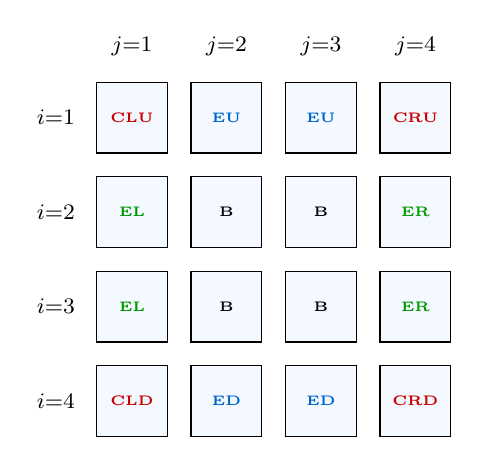
\begin{tikzpicture}[scale=1.2, font=\small]
  % Draw grid
  \foreach \i in {1,...,4} {
    \foreach \j in {1,...,4} {
      \node[draw, minimum size=0.9cm, fill=lightblue!30] at (\j, 5-\i) {};
    }
  }

  % Labels
  \node[above] at (1, 4.55) {\footnotesize $j{=}1$};
  \node[above] at (2, 4.55) {\footnotesize $j{=}2$};
  \node[above] at (3, 4.55) {\footnotesize $j{=}3$};
  \node[above] at (4, 4.55) {\footnotesize $j{=}4$};
  \node[left] at (0.5, 4) {\footnotesize $i{=}1$};
  \node[left] at (0.5, 3) {\footnotesize $i{=}2$};
  \node[left] at (0.5, 2) {\footnotesize $i{=}3$};
  \node[left] at (0.5, 1) {\footnotesize $i{=}4$};

  % Corner labels
  \node[font=\tiny\bfseries, text=myred] at (1, 4) {CLU};
  \node[font=\tiny\bfseries, text=myblue] at (2, 4) {EU};
  \node[font=\tiny\bfseries, text=myblue] at (3, 4) {EU};
  \node[font=\tiny\bfseries, text=myred] at (4, 4) {CRU};
  \node[font=\tiny\bfseries, text=mygreen] at (1, 3) {EL};
  \node[font=\tiny\bfseries] at (2, 3) {B};
  \node[font=\tiny\bfseries] at (3, 3) {B};
  \node[font=\tiny\bfseries, text=mygreen] at (4, 3) {ER};
  \node[font=\tiny\bfseries, text=mygreen] at (1, 2) {EL};
  \node[font=\tiny\bfseries] at (2, 2) {B};
  \node[font=\tiny\bfseries] at (3, 2) {B};
  \node[font=\tiny\bfseries, text=mygreen] at (4, 2) {ER};
  \node[font=\tiny\bfseries, text=myred] at (1, 1) {CLD};
  \node[font=\tiny\bfseries, text=myblue] at (2, 1) {ED};
  \node[font=\tiny\bfseries, text=myblue] at (3, 1) {ED};
  \node[font=\tiny\bfseries, text=myred] at (4, 1) {CRD};
\end{tikzpicture}
\end{center}

\begin{center}
\renewcommand{\arraystretch}{1.3}
\begin{tabular}{ll}
\toprule
格点类型 & 需收缩的键 \\
\midrule
\textbf{B}（内部） & 无收缩，9 指标张量保持原样 \\
\textbf{EU}（上边缘） & $u \leftarrow \mathbf{v}_0$（列起始），$ul \leftarrow \mathbf{v}_0$（$\searrow$ 起始），$ru \leftarrow$ 见下 \\
\textbf{ED}（下边缘） & $d \leftarrow \mathbf{v}_1$（列终止），$dr \leftarrow$ 见下，$ld \leftarrow$ 见下 \\
\textbf{EL}（左边缘） & $l \leftarrow \mathbf{v}_0$（行起始），$ul \leftarrow \mathbf{v}_0$（$\searrow$ 起始），$ld \leftarrow \mathbf{v}_0$（$\nearrow$ 起始） \\
\textbf{ER}（右边缘） & $r \leftarrow \mathbf{v}_1$（行终止），$dr \leftarrow \mathbf{v}_2$（$\searrow$ 终止），$ru \leftarrow \mathbf{v}_2$（$\nearrow$ 终止） \\
\textbf{CLU}（左上角） & $u, ul, l, ld \leftarrow \mathbf{v}_0$；$ru$ 根据反对角线 \\
\textbf{CRU}（右上角） & $u \leftarrow \mathbf{v}_0$；$r \leftarrow \mathbf{v}_1$；$ru \leftarrow \mathbf{v}_2$；$ul \leftarrow \mathbf{v}_0$ \\
\bottomrule
\end{tabular}
\end{center}

\subsection{具体例子：左上角格点 $(1,1)$}

以 $4 \times 4$ 棋盘的左上角为例，详细展示边界收缩过程。

格点 $(1,1)$ 的 4 条约束线：
\begin{itemize}
  \item \textbf{列}：第 1 列的起点 $\to$ $u \leftarrow \mathbf{v}_0$，固定 $u = 0$
  \item \textbf{行}：第 1 行的起点 $\to$ $l \leftarrow \mathbf{v}_0$，固定 $l = 0$
  \item \textbf{$\searrow$ 对角线}：主对角线的起点 $\to$ $ul \leftarrow \mathbf{v}_0$，固定 $ul = 0$
  \item \textbf{$\nearrow$ 反对角线}：长度为 1 的对角线（只有这一个格点）$\to$ $ld \leftarrow \mathbf{v}_0$ 且 $ru \leftarrow \mathbf{v}_2$
\end{itemize}

收缩 $\mathbf{v}_0$ 固定入方向为 0；收缩 $\mathbf{v}_2$ 对出方向求和（$0 + 1$）。经过所有收缩后：

\begin{sumbox}[左上角的有效张量]
只剩下 3 个自由键指标：$d, dr, r$。有效张量为：
\begin{align*}
T_{1,1}^{\text{eff}}(d, dr, r) &= \sum_{ru=0}^{1} T(0, d, 0, r, 0, dr, 0, ru, p{=}0) + T(0, d, 0, r, 0, dr, 0, ru, p{=}1) \\
&= \sum_{ru} A^{0,d}(p) \cdot A^{0,r}(p) \cdot A^{0,dr}(p) \cdot A^{0,ru}(p) \cdot V_0(p)
\end{align*}
其中 $V_0(p) = 1$（对 $p$ 求和，因为 $\hat{n}_0 + \hat{n}_1 = \mathbb{I}$）。

\medskip
非零元素只有 2 个：
\begin{center}
\renewcommand{\arraystretch}{1.2}
\begin{tabular}{ccc|c|l}
\toprule
$d$ & $dr$ & $r$ & 值 & 含义 \\
\midrule
$0$ & $0$ & $0$ & $1$ & 空格子，无信号 \\
$1$ & $1$ & $1$ & $1$ & 放皇后，向 $d, dr, r$ 发信号 \\
\bottomrule
\end{tabular}
\end{center}
这与旧方法中 $T_{1,1}$ 的 2 个有效自由度完全吻合（对应旧方法 $8 \times 4$ 矩阵中的 4 个非零元素，但合并对角线编码后恰好是 2 个物理独立状态）。
\end{sumbox}

\subsection{对比：新方法 vs 旧方法的边界处理}

\begin{center}
\renewcommand{\arraystretch}{1.3}
\begin{tabular}{p{5cm}p{5cm}}
\toprule
\textbf{旧方法} & \textbf{新方法} \\
\midrule
手动设置边界 $B$ 张量的指标维度为 1 & 收缩 $\mathbf{v}_0$ 或 $\mathbf{v}_1/\mathbf{v}_2$，自动降维 \\
需要 UE（编码器）把对角线信号合并到水平键 & 对角线键直接存在，边界自然收缩 \\
需要 DE（解码器）从垂直键拆分对角线信号 & 不需要——对角线键独立传播 \\
需要 V0 对物理指标求和 & 可选：用 $\hat{n}_0 + \hat{n}_1 = \mathbb{I}$ 或等价地乘以 $(|0\rangle + |1\rangle)$ \\
边界张量有 7 种类型（CLU, CRU, CLD, CRD, EU, ED, EL, ER）需分别编码 & 所有格点用\textbf{同一个} $T$ 张量，边界条件通过向量收缩实现 \\
\bottomrule
\end{tabular}
\end{center}

%=============================================================================
\section{完整的配分函数}
%=============================================================================

\subsection{量子态的构造}

配分函数 $Z_N$（即 N 皇后问题的解数）可以用以下方式计算：

\begin{keybox}[配分函数]
\[
Z_N = \langle \Psi | \left( |0\rangle + |1\rangle \right)^{\otimes N^2}
\]
其中 $|\Psi\rangle$ 由所有格点的 T 张量（经过边界收缩）的张量网络定义：
\[
|\Psi\rangle = T^{\alpha\alpha'}_{i_1 j_1 k_1 l_1, i'_1 j'_1 k'_1 l'_1} \cdot \left( |0\rangle + |1\rangle \right)^{\otimes N^2}
\]
$\left( |0\rangle + |1\rangle \right)$ 的作用是对每个格点的物理指标求和（遍历所有可能的占据配置），等价于旧方法中 V0 张量的功能。
\end{keybox}

\subsection{张量网络图}

整个 $N \times N$ 棋盘形成一个二维张量网络：

\begin{center}
\begin{tikzpicture}[scale=1.4, font=\small]
  % Draw tensors
  \foreach \i in {1,...,4} {
    \foreach \j in {1,...,4} {
      \node[draw, fill=lightblue, minimum size=0.6cm, rounded corners=2pt, inner sep=0pt]
        (T\i\j) at (\j, 5-\i) {\tiny $T_{\i,\j}$};
    }
  }

  % Horizontal bonds (row constraints)
  \foreach \i in {1,...,4} {
    \foreach \j in {1,...,3} {
      \pgfmathtruncatemacro{\jnext}{\j+1}
      \draw[thick, myred] (T\i\j) -- (T\i\jnext);
    }
  }

  % Vertical bonds (column constraints)
  \foreach \j in {1,...,4} {
    \foreach \i in {1,...,3} {
      \pgfmathtruncatemacro{\inext}{\i+1}
      \draw[thick, myblue] (T\i\j) -- (T\inext\j);
    }
  }

  % Main diagonal bonds
  \foreach \i in {1,...,3} {
    \foreach \j in {1,...,3} {
      \pgfmathtruncatemacro{\inext}{\i+1}
      \pgfmathtruncatemacro{\jnext}{\j+1}
      \draw[thick, mygreen, dashed] (T\i\j) -- (T\inext\jnext);
    }
  }

  % Anti-diagonal bonds
  \foreach \i in {2,...,4} {
    \foreach \j in {1,...,3} {
      \pgfmathtruncatemacro{\iprev}{\i-1}
      \pgfmathtruncatemacro{\jnext}{\j+1}
      \draw[thick, mypurple, dotted] (T\i\j) -- (T\iprev\jnext);
    }
  }

  % Boundary vectors (示意)
  \foreach \j in {1,...,4} {
    \draw[-{Stealth}, thick, myblue!50] (T1\j.north) -- ++(0, 0.3) node[above] {\tiny $\mathbf{v}_0$};
    \draw[-{Stealth}, thick, myblue!50] (T4\j.south) -- ++(0, -0.3) node[below] {\tiny $\mathbf{v}_1$};
  }
  \foreach \i in {1,...,4} {
    \draw[-{Stealth}, thick, myred!50] (T\i1.west) -- ++(-0.3, 0) node[left] {\tiny $\mathbf{v}_0$};
    \draw[-{Stealth}, thick, myred!50] (T\i4.east) -- ++(0.3, 0) node[right] {\tiny $\mathbf{v}_1$};
  }

  % Legend
  \node[anchor=west] at (5.3, 4.2) {\small \color{myred}\textbf{---} 行键};
  \node[anchor=west] at (5.3, 3.7) {\small \color{myblue}\textbf{---} 列键};
  \node[anchor=west] at (5.3, 3.2) {\small \color{mygreen}\textbf{- -} $\searrow$ 对角线键};
  \node[anchor=west] at (5.3, 2.7) {\small \color{mypurple}\textbf{$\cdots$} $\nearrow$ 反对角线键};
\end{tikzpicture}
\end{center}

\begin{warnbox}[注意：对角线使网络非平面]
对角线键（绿色虚线和紫色点线）使得张量网络不再是简单的正方格子。这正是需要将对角线键编码进水平/垂直键（旧方法中 UE/DE 的作用）才能用 MPS/MPO 方法处理的原因。

新方法的 T 张量保留了对角线键的独立性，从概念上更清晰。要实际用 MPS/MPO 计算，仍需将对角线合并进上下左右键中，但\textbf{构造过程}变得更透明。
\end{warnbox}

\subsection{从 T 张量到可计算的网络张量}

要用 MPS/MPO 方法计算，需要将 9 指标的 T 张量转化为只有上下左右 4 个方向键的网络张量（即旧方法中的 $T_{i,j}$）。步骤是：
\begin{enumerate}
  \item 对 $p$ 指标收缩 $(|0\rangle + |1\rangle)$：等价于对 $p = 0$ 和 $p = 1$ 求和
  \item 将对角线键 $(ul, dr)$ 编码进垂直和水平键：$ul \to$ 上行水平键，$dr \to$ 下行垂直键（UE/DE 的功能）
  \item 边界格点收缩边界向量
  \item Reshape 合并指标，得到最终的 $[\chi_{\text{up}}, \chi_{\text{down}}, \chi_{\text{left}}, \chi_{\text{right}}]$ 张量
\end{enumerate}

最终得到的网络张量与旧方法完全相同，但推导过程更加系统化。

%=============================================================================
\section{推广到任意 $N$}
%=============================================================================

新方法的一大优势是构造过程与 $N$ 无关：

\begin{keybox}[$N \times N$ 棋盘的构造步骤]
\begin{enumerate}
  \item 定义转移矩阵 $A = \begin{pmatrix} \hat{n}_0 & \hat{n}_1 \\ 0 & \hat{n}_0 \end{pmatrix}$（与 $N$ 无关）

  \item 对每个格点 $(i,j)$，T 张量公式不变：
  \[
  T(u, d, l, r, ul, dr, ld, ru, p) = A^{ud}(p) \cdot A^{lr}(p) \cdot A^{ul,dr}(p) \cdot A^{ld,ru}(p)
  \]

  \item 确定每个格点处哪些键需要收缩边界向量：
  \begin{itemize}
    \item 约束线的\textbf{起点}处：收缩 $\mathbf{v}_0 = (1, 0)$
    \item 行/列约束的\textbf{终点}处：收缩 $\mathbf{v}_1 = (0, 1)$
    \item 对角线约束的\textbf{终点}处：收缩 $\mathbf{v}_2 = (1, 1)$
  \end{itemize}

  \item 收缩所有键指标，得到配分函数 $Z_N$
\end{enumerate}
\end{keybox}

对于任意 $N$，T 张量的内部结构（17 个非零元素）完全不变——变化的只是网络的大小和边界收缩的位置。

%=============================================================================
\section{总结与对比}
%=============================================================================

\begin{sumbox}[新旧方法对比总结]
\begin{center}
\renewcommand{\arraystretch}{1.4}
\begin{tabular}{p{3cm}p{4.5cm}p{4.5cm}}
\toprule
& \textbf{旧方法} & \textbf{新方法（转移矩阵法）} \\
\midrule
核心对象 & 9 阶 $B$ 张量 & 转移矩阵 $A$（$2 \times 2$，元素为算符） \\
17 个非零元素 & 手动逐一列出 & 从 $A$ 自动推导：$T = A \cdot A \cdot A \cdot A$ \\
物理直觉 & 需理解 9 个指标的组合 & $A$ 的上三角结构 = 信号只增不减 \\
边界条件 & 需 UE/DE/V0 辅助张量 & 三个向量 $\mathbf{v}_0, \mathbf{v}_1, \mathbf{v}_2$ \\
推广性 & 需为每种边界类型单独编码 & 统一公式，自动处理 \\
MPS/MPO 转化 & 内建（UE/DE 已完成编码） & 需额外步骤合并对角线键 \\
\bottomrule
\end{tabular}
\end{center}
\end{sumbox}

\begin{keybox}[一句话总结]
N 皇后问题的局部张量 $T$ 就是 4 个转移矩阵 $A$ 的元素之乘积——每条经过该格点的约束线贡献一个 $A$。边界条件通过 $\mathbf{v}_0$（起始）、$\mathbf{v}_1$（恰好一个）、$\mathbf{v}_2$（至多一个）三个向量的收缩自动完成。这一构造与棋盘大小 $N$ 无关，是最自然、最系统的方式。
\end{keybox}

\end{document}
